\documentclass[11pt]{article}
\usepackage[margin=1in]{geometry}
\usepackage[T1]{fontenc}
\usepackage{lmodern}
\usepackage{amsmath,amssymb,booktabs,array,longtable,graphicx}
\newcolumntype{L}[1]{>{\raggedright\arraybackslash}p{#1}}
\usepackage{hyperref}
\setlength{\emergencystretch}{8em}
\renewcommand{\arraystretch}{1.3}
\makeatletter
\newcommand{\sha}{\begingroup\catcode`\_=12 \sha@read}
\newcommand{\sha@read}[1]{\ttfamily\sha@loop#1\relax\endgroup}
\def\sha@loop#1{%
  \ifx\relax#1\else
    #1\allowbreak
    \expandafter\sha@loop
  \fi}
\makeatother
\hypersetup{colorlinks=true,linkcolor=blue,urlcolor=blue,citecolor=blue,
  pdftitle={Replication of the autobiographical-memory tests in Sorenson (2015)},
  pdfauthor={}}
\newcommand{\proofcommit}{8464d95399f8f05c6944c3997efd3cef934fd861}
\makeatletter
\def\ogm@show#1{%
  \ifx\relax#1\else
    #1\allowbreak
    \expandafter\ogm@show
  \fi}
\newcommand{\src}{\begingroup\catcode`\_=12 \ogm@src}
\newcommand{\ogm@src}[1]{%
  \edef\srcurl{https://github.com/alectionary/vibe-math/blob/master/formalization/overgeneral-memory/#1}%
  \href{\srcurl}{\texttt{\ogm@show#1\relax}}\endgroup}
\newcommand{\srcat}{\begingroup\catcode`\_=12 \ogm@srcat}
\newcommand{\ogm@srcat}[2]{%
  \edef\srcurl{https://github.com/alectionary/vibe-math/blob/master/formalization/overgeneral-memory/#1\#L#2}%
  \href{\srcurl}{\texttt{\ogm@show#1\relax}}\endgroup}
\makeatother

\title{Replication of the autobiographical-memory tests\\
in Sorenson (2015)}
\author{}
\date{29 October 2026}

\begin{document}
\maketitle

\begin{abstract}
Do adults with major depression give fewer specific autobiographical memories
than adults who are not depressed, and do the printed tests in Sorenson
(2015) follow from the printed means, standard deviations, and sample sizes?
Sorenson reports a trend toward fewer specific memories in the depressed
group, \(t(35) = 1.96\), \(p = .058\), no comparable impairment on a
paired-associate recall test, and lower right prefrontal activity during
successful image retrieval, with that cluster correlated with
autobiographical specificity at \(r = .46\).
The tests fixed by the printed moments were recomputed in R, and the
printed questionnaire means were checked as averages of integer scores.
The specificity trend is recovered at the stated final sizes, 20 and 17:
the moments give \(t = 1.95\), the printed \(1.96\) lies in the half-digit
band \(1.93\) to \(1.98\), and the two-tailed \(p\)-value of \(t(35) = 1.96\)
is \(.058\).
The Beck depression statistic \(10.94\) matches the recruited sizes 20 and
19, while the printed degrees of freedom \(35\) match the final sizes, where
the same moments give \(t = 10.36\).
The negative-mood statistic \(4.5\) lies outside the half-digit band at 20
and 17 and is recovered at 19 and 18, the sizes at which those mood means
are possible averages of integer scores.
The right prefrontal cluster was not recomputed.
No images or region summaries are public, and the \(p\)-value attached to
\(r = .46\) agrees with a correlation of that size in this sample.
\end{abstract}

\section{The question and the headline result}
\label{sec:headline}

This section answers what Sorenson tested and what happened to that result
here.
The dissertation asks whether overgeneral autobiographical memory in major
depression is tied to abnormal neural activity when a paired image is
retrieved.
The headline behavioral result is a trend: depressed participants produced
fewer specific memories than nondepressed participants.
The headline neural result is lower activity in the right middle frontal
gyrus during successful retrieval, in the depressed group, together with a
positive correlation between that activity and autobiographical specificity.
The specificity trend matches the printed moments.
The cluster itself remains unchecked, because the images are not public.

Sorenson~\cite{sorenson2015} tested 20 depressed and 19 nondepressed adults,
then excluded two nondepressed participants, and analyzed a final sample of
20 and 17.
Everyone took the Autobiographical Memory Test and, in the scanner, a
paired-associate task that linked concrete nouns to famous faces and places.
Table~\ref{tab:compare} is the comparison.
A match means the printed statistic is the value computed from the printed
moments, or it lies inside the half-digit bin defined in
Section~\ref{sec:assumptions}.
These checks are tail probabilities of printed moments.
Agreement is the half-digit bin of those moments.
A two-standard-error simulation band, and Bonferroni or Holm on such a
band, applies to Monte Carlo rates, which this note does not estimate.

The specificity means are \(10.80\) (SD \(1.64\)) and \(11.82\) (SD \(1.51\)).
At \(n = 20\) and \(n = 17\), \srcat{simulation/recompute.R}{37} gives
\(t = -1.9546\), two-tailed \(p = .059\).
The page prints the unsigned \(t(35) = 1.96\), and the prose says the
depressed mean is the lower one.
The half-digit band on those four moments runs from \(1.93\) to \(1.98\) in
absolute value, which contains \(1.96\).
The two-tailed \(p\)-value of the printed \(t(35) = 1.96\) is \(.0580\).
The group \(F(1, 35) = 3.84\) is the square of that printed \(t\)
(\(1.96^2 = 3.8416\)).
Figure~\ref{fig:amt} is the paragraph.
The right prefrontal cluster in Table~8 of the dissertation, 220 voxels,
was not recomputed.
The correlation of that cluster with specificity is \(r = .46\), \(p < .01\).
At \(N = 37\), \srcat{simulation/recompute.R}{156} gives \(p = .0042\) for a
correlation of that size.
At \(N = 36\), allowing the participant whose clarity ratings were missing,
\(p = .0048\).

\begin{figure}[ht]
\centering
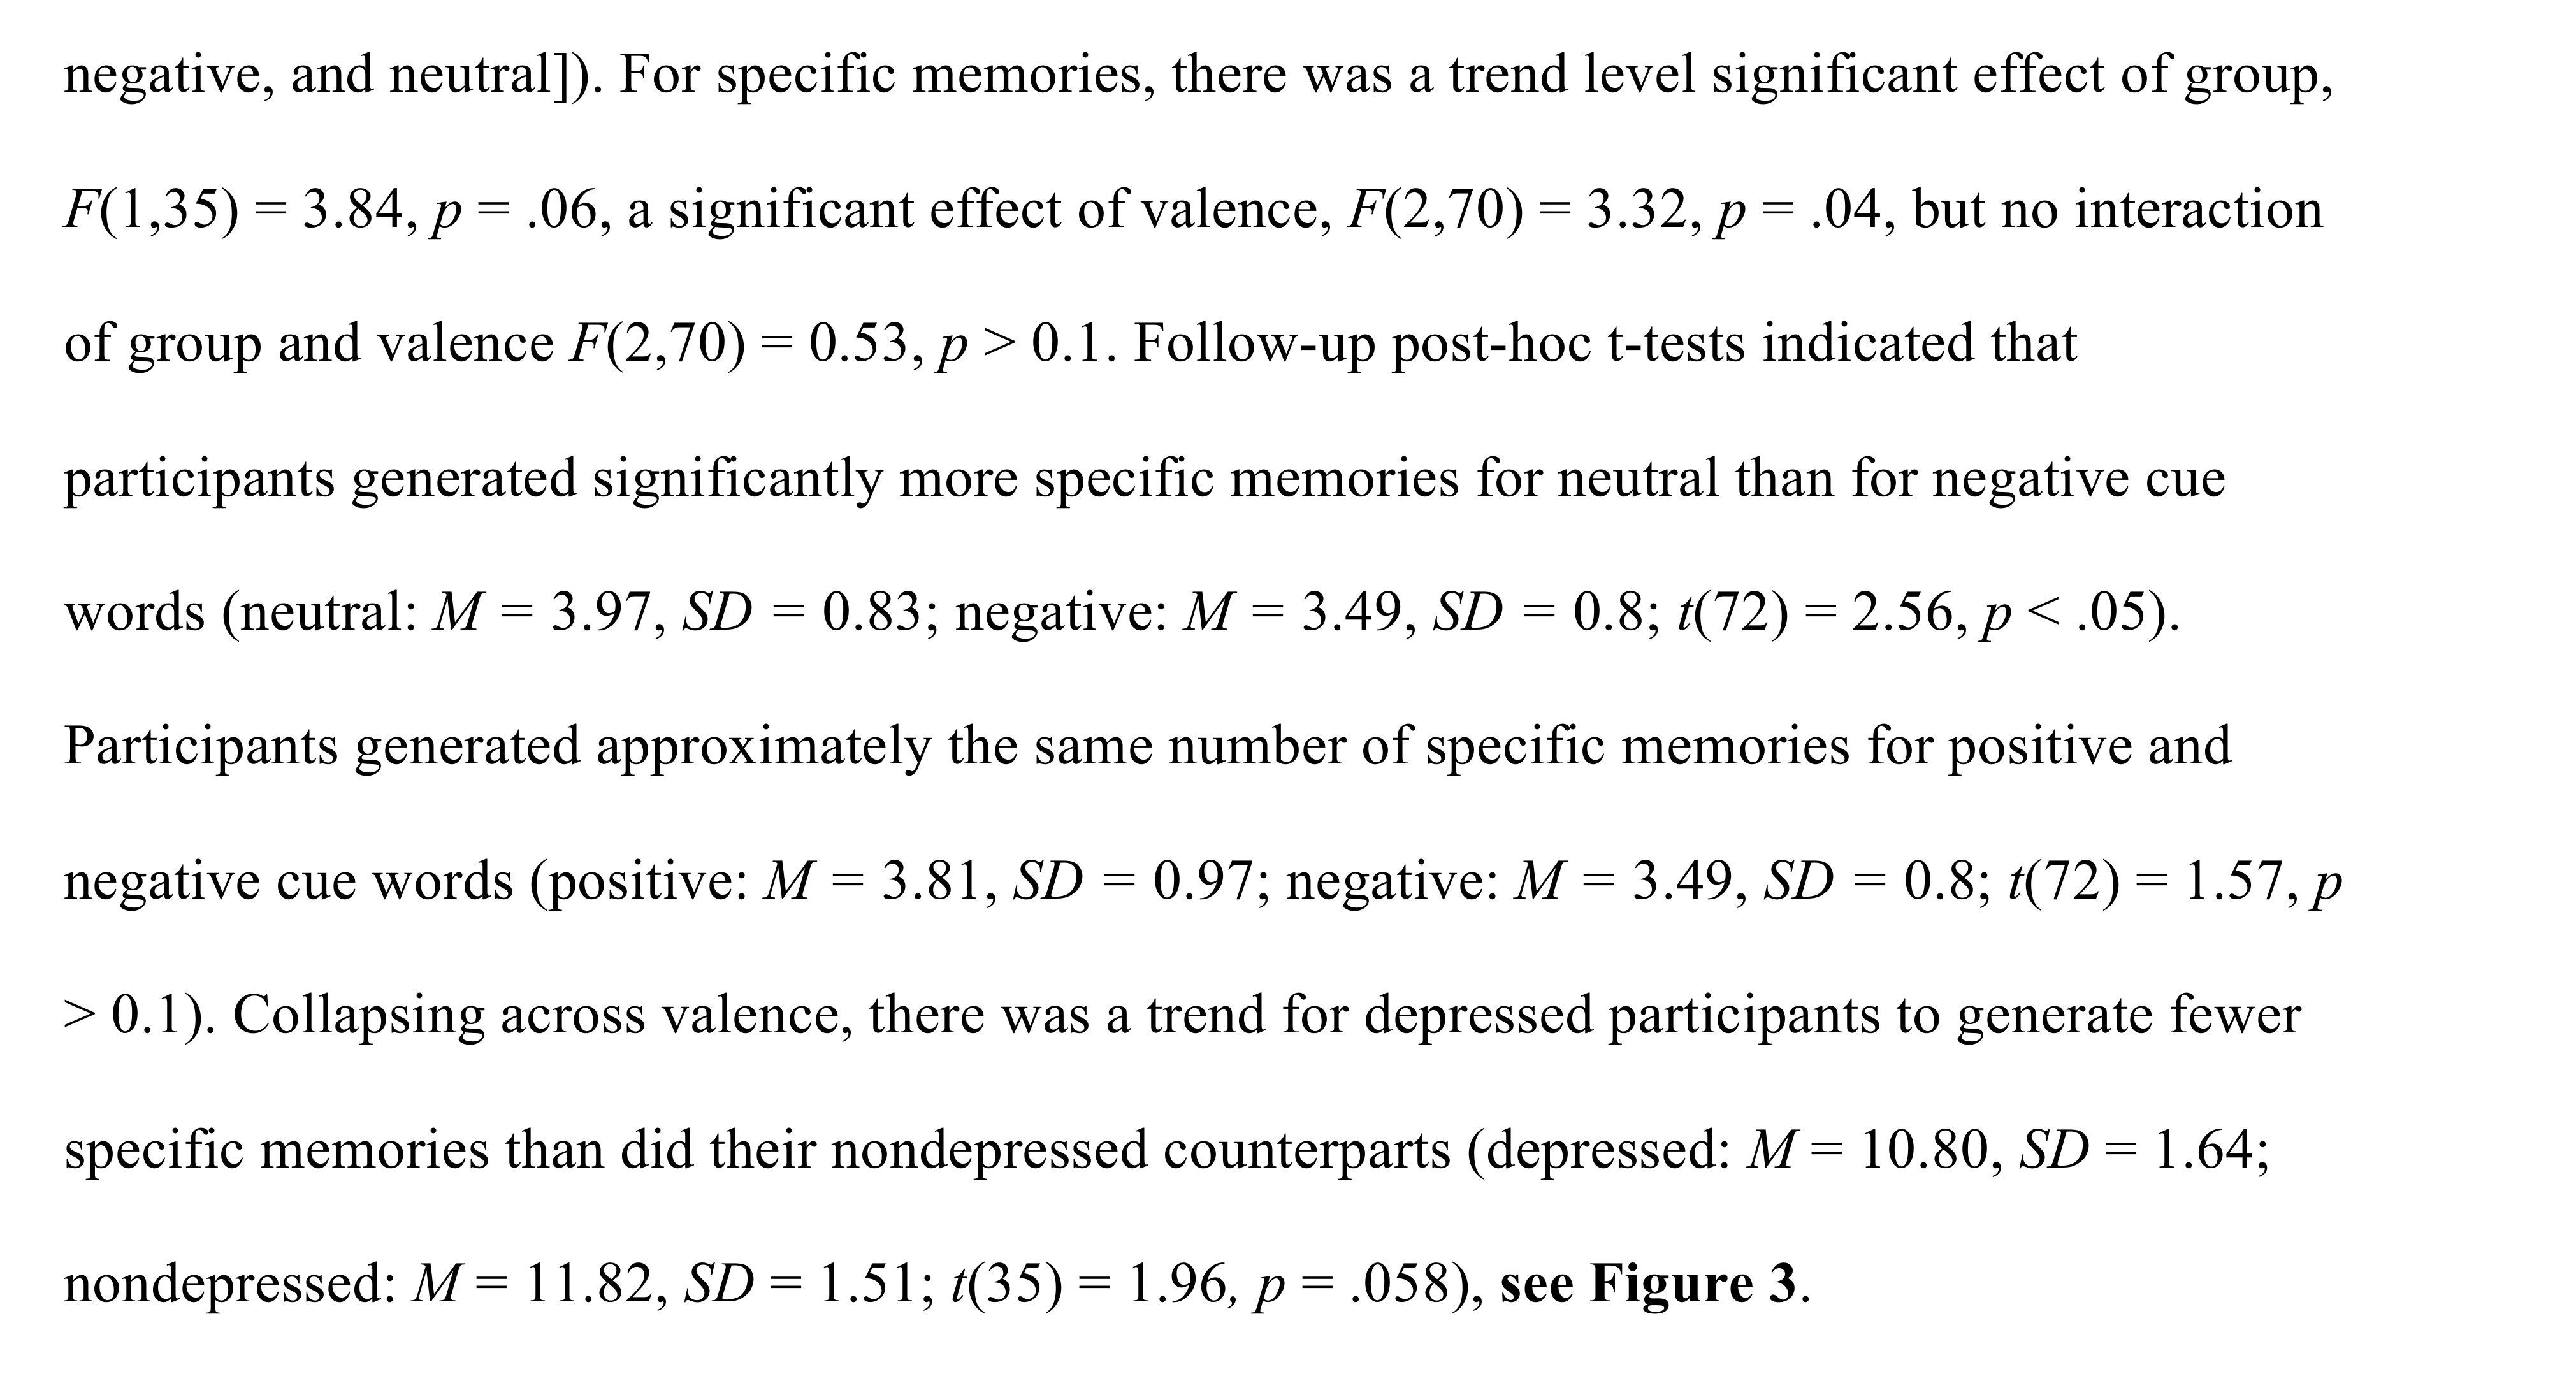
\includegraphics[width=\textwidth]{figures/amt-tests.png}
\caption{Autobiographical Memory Test statistics on dissertation page~28
(PDF page~36), rendered at 600 dpi.
The group test is \(F(1,35) = 3.84\), \(p = .06\), and the collapsed test is
\(t(35) = 1.96\), \(p = .058\).}
\label{fig:amt}
\end{figure}

\section{What we did ourselves, and what we took from others}
\label{sec:did}

This section answers which numbers are ours and which are Sorenson's.
Sorenson's contribution is the design, the sample, and the printed tables.
Our contribution is the recomputation in Table~\ref{tab:compare}, the
integer-score checks, the page crops, and the derived effect sizes, which
the dissertation does not print.
Every later number is one of those three: our calculation, an assumption in
Section~\ref{sec:assumptions}, or a figure taken from the dissertation.

R~4.3.3~\cite{rcore} is the implementation of the \(t\), \(F\), chi-square,
and correlation tails.
The dissertation names AFNI, FreeSurfer, nilearn, scikit-learn, and Praat
for imaging and for the timing of spoken recall.
It does not name the program that produced the behavioral \(t\) and \(F\)
tests, so there is no original version to match.
Base R is sufficient: the formulas do not depend on a contributed statistics
package.
jsonlite~1.8.8~\cite{jsonlite} writes the JSON files.
The test formulas are base R.
Poppler~24.02.0~\cite{poppler} renders the pages and reads the text layer,
because a comma and a period have to be compared on the page, not only in
the extracted string.
Python~3.12.3~\cite{python} and Pillow~10.2.0~\cite{pillow} cut those
rasters at the word boxes.
pdf\TeX, \TeX~Live~2023~\cite{texlive}, typesets this note.
Welch's \(t\), \srcat{simulation/recompute.R}{50}, is the second variance
formula, used where the Student reading and the printed statistic separate.

The dissertation file is the Stanford Digital Repository PDF, 91 pages,
sha256
\sha{4debc9f5551d51ae00a5b6987c3c572a9c7221f6ab631928558c8c1f6b8414d6}.
It is not in git.
The crops in \src{paper/figures/} are the page images this note relies on.

\section{What the recomputed tests say}
\label{sec:table}

This section answers which printed tests follow from the printed moments.
Table~\ref{tab:compare} is that comparison.
The paragraphs under the table give one reason for each row.
Moments, degrees of freedom, and \(p\)-values are in
\src{simulation/out/claims.json}, written by
\srcat{simulation/recompute.R}{37}.

\begin{footnotesize}
\begin{longtable}{@{}L{0.22\textwidth}L{0.24\textwidth}L{0.32\textwidth}L{0.12\textwidth}@{}}
\caption{Published claims and our calculations.
Unsigned \(t\) statistics are compared in absolute value.
The prose of the dissertation gives the direction.}
\label{tab:compare}\\
\toprule
Claim & Published & Ours & Verdict \\
\midrule
\endfirsthead
\toprule
Claim & Published & Ours & Verdict \\
\midrule
\endhead
Specific memories, group \(t\) &
\(t(35)=1.96\), \(p=.058\) &
\(t=1.955\), \(p=.059\); band \(1.93\) to \(1.98\) &
match \\
Specific memories, group \(F\) &
\(F(1,35)=3.84\), \(p=.06\) &
\(1.96^2=3.842\); \(p=.058\) &
match \\
Valence error degrees of freedom &
\(F(2,70)\) &
\((3-1)(37-2)=70\) &
match \\
Valence main effect &
\(F(2,70)=3.32\), \(p=.04\) &
\(p=.042\); \(F\) not recomputed &
partial \\
Group by valence &
\(F(2,70)=0.53\), \(p>0.1\) &
\(p=.591\); \(F\) not recomputed &
partial \\
Neutral versus negative cues &
\(t(72)=2.56\), \(p<.05\) &
\(t=2.533\), \(p=.013\); band \(2.46\) to \(2.60\) &
match \\
Positive versus negative cues &
\(t(72)=1.57\), \(p>0.1\) &
\(t=1.548\), \(p=.126\); band \(1.49\) to \(1.61\) &
match \\
Gender &
\(\chi^2(1,N=39)=0.20\), \(p>0.1\) &
Pearson \(0.208\), \(p=.65\) &
close \\
Age &
\(t(37)=0.08\), \(p>0.1\) &
\(t=-0.080\), \(p=.94\) &
match \\
Years of education &
\(t(37)=1.12\), \(p>.1\) &
\(t=-1.120\), \(p=.27\) &
match \\
Handedness &
\(\chi^2(1,N=39)=0.98\), \(p>0.1\) &
\(2\times 3\) Pearson \(0.975\), df \(2\), \(p=.61\) &
partial \\
Shipley vocabulary &
\(t(36)=0.55\), \(p>.1\) &
\(0.554\) at \(19/19\); \(0.557\) at \(20/18\) &
close \\
Beck depression inventory &
\(t(35)=10.94\), \(p<0.001\) &
\(10.94\) at \(20/19\) (df \(37\)); \(10.36\) at \(20/17\) (df \(35\)) &
partial \\
Positive mood, stated sizes &
\(t(35)=1.81\), \(p=.08\) &
\(t=-1.804\), \(p=.080\); band to \(-1.809\) &
close \\
Negative mood, stated sizes &
\(t(35)=4.5\), \(p<0.001\) &
\(t=4.414\), \(p=9.3\times 10^{-5}\); band \(4.40\) to \(4.43\) &
no match \\
Both mood scales, \(n=19\) and \(18\) &
\(t(35)=1.81\) and \(t(35)=4.5\) &
\(t=-1.811\), \(p=.079\); \(t=4.516\), \(p=6.9\times 10^{-5}\) &
match \\
In-scanner clarity, group \(t\) &
\(t(35)=0.17\), \(p>0.1\) &
\(t=0\) at the printed means; band \(-0.49\) to \(0.49\) &
match \\
Clarity, later hit versus miss &
\(t(36)=13.08\), \(p<0.001\) &
\(p=3.0\times 10^{-15}\); feasible \(|t|\) in \([6.7, 29.7]\) &
partial \\
Subsequent-memory \(F\) denominator &
\(F(1,105)=379.55\), \(p<0.001\) &
\(37\times 3-6=105\); \(p\) of the printed \(F\) is \(<0.001\) &
partial \\
Reward \(F\), decimal comma &
\(F(1,35)=2{,}97\), \(p=0.09\) &
\(p=.094\) for \(F=2.97\); \(p\) near \(0\) for \(F=297\) &
match \\
Reward, paired follow-up &
\(t(36)=1.80\), \(p=0.08\) &
\(p=.080\); feasible \(|t|\) in \([0.38, 4.06]\) &
partial \\
Specific hits, group \(F\) &
\(F(1,35)=0.01\), \(p>0.1\) &
\(p=.92\); \(F\) not recomputed &
partial \\
Reaction-time degrees of freedom &
\(F(1,36)\) three times &
\(p=.28\), \(1\), \(.65\); the hits tests use df \(35\) &
partial \\
General hits &
\(t(35)=1.57\), \(p>0.1\) &
\(t=1.569\), \(p=.126\) &
match \\
ROI voxel count &
\(t(35)=0.07\), \(p>0.1\) &
\(t=0.075\), which rounds to \(0.07\); \(p=.94\) &
match \\
Encoding classification &
\(t(35)=1.26\), \(p>0.1\) &
\(t=1.237\), \(p=.22\); band \(1.14\) to \(1.33\) &
match \\
Reinstatement above chance &
\(t(36)=13.54\), \(p<.01\) &
\(t=13.65\), \(p\) near \(0\); band \(13.52\) to \(13.77\) &
match \\
Reinstatement, group \(t\) &
\(t(35)=1.89\), \(p=0.073\) &
\(t=1.842\), \(p=.074\); band \(1.79\) to \(1.89\) &
close \\
General hits with specificity &
\(r=-.36\), \(p<0.05\) &
\(p=.029\) at \(N=37\) &
match \\
Classifier with specificity &
\(r=-0.33\), \(p<0.05\) &
\(p=.046\) at \(N=37\); \(p=.049\) at \(N=36\) &
match \\
Right middle frontal gyrus with specificity &
\(r=.46\), \(p<.01\) &
\(p=.004\) at \(N=37\); \(p=.005\) at \(N=36\) &
match \\
Two near-zero correlations &
\(r=.03\) and \(r=-0.03\), \(p>0.1\) &
\(p=.86\) and \(p=.86\) at \(N=37\) &
match \\
\bottomrule
\end{longtable}
\end{footnotesize}

The specificity \(t\) row is the headline.
The moments at 20 and 17 produce \(1.95\), and \(1.96\) is inside the
half-digit band.
The specificity \(F\) row is that same contrast: the printed \(F\) is the
square of the printed \(t\), and its \(p\)-value prints as \(.06\) where the
\(t\) prints as \(.058\).
The valence degrees-of-freedom row is the within-subject error of a
three-level factor in a two-group sample of 37, which is 70.
The valence \(F\) row and the interaction row agree in the tail probability
of the printed \(F\), and the \(F\) itself is not determined by the three
marginal means.
The two cue-contrast rows use an independent-samples \(t\) on 37 and 37,
which is what \(t(72)\) states.
Reading the negative-cue standard deviation as \(0.80\) rather than as the
one-decimal \(0.8\), both printed \(t\) values sit in the half-digit band.

The gender row is Pearson's chi-square on the printed counts 13, 7, 11, and
8, without the continuity correction.
The statistic is \(0.208\).
Yates's correction, the alternative tried in
Section~\ref{sec:trouble}, gives \(0.016\).
The age and education rows use the recruited sizes 20 and 19, because
\(t(37)\) is \(n_1+n_2-2\) for those sizes, and the absolute values round to
the printed statistics.
The depressed means are the lower ones, so the signed statistics are
negative.
The handedness row is the \(2\times 3\) table of right, left, and
ambidextrous, whose Pearson statistic \(0.975\) rounds to the printed
\(0.98\), on 2 degrees of freedom.
The printed degrees of freedom are 1.
Collapsing ambidextrous into ``not right'' gives \(0.17\), which is not
\(0.98\).

The Shipley row has two nearby splits that share \(t(36)\).
Equal sizes 19 and 19 give \(t = 0.554\), which rounds to \(0.55\).
The integer-consistent sizes 20 and 18 give \(t = 0.557\), which rounds to
\(0.56\).
Section~\ref{sec:trouble} records which of those means can be integer
totals.
The Beck row splits the same way across samples: \(10.938\) at the recruited
20 and 19, and \(10.360\) at the final 20 and 17.
Welch's formula gives \(11.20\) and \(11.16\) on those two splits.
The positive-mood row at the stated 20 and 17 is \(1.804\), and the
half-digit band reaches \(1.809\), just short of the printed \(1.81\).
The \(p\)-value \(.080\) prints as \(.08\).
The negative-mood row at those sizes is \(4.414\).
The half-digit band is \(4.401\) to \(4.427\), and the printed \(4.5\) lies
outside it.
The inequality \(p < 0.001\) holds for \(4.414\)
(\(p = 9.3\times 10^{-5}\)).
The mood row at 19 and 18 is the sample that is integer-consistent for both
scales and that reproduces both printed \(t\) statistics on 35 degrees of
freedom.
That sample size is an assumption we supplied.
It is not a size the dissertation states.

The clarity row treats the two printed means \(3.9\) and \(3.9\) as exact and
gets \(t = 0\).
The printed \(0.17\) lies inside the one-decimal band on those means.
The later-hit row checks the printed \(t(36) = 13.08\): its \(p\)-value is
far below \(.001\), and the marginal moments allow a paired \(t\) between
\(6.7\) and \(29.7\).
The implied correlation of hit and miss clarity, if the printed \(t\) and the
printed marginal standard deviations are exact, is \(0.55\).
The subsequent-memory denominator row is the arithmetic
\(37\times 3 - 6 = 105\), derived in Section~\ref{sec:resolved}.
The \(F\) of \(379.55\) was not recomputed.
The reward \(F\) row reads the printed comma as a decimal comma, because
\(F(1,35) = 2.97\) has \(p = .094\), which prints as \(0.09\), and
\(F = 297\) has a \(p\)-value near 0.
Figure~\ref{fig:comma} is that mark.
The reward follow-up is feasible: the implied correlation of high-reward and
low-reward hit counts is \(0.93\), inside \((-1, 1)\), and the \(p\)-value of
\(t(36) = 1.80\) is \(.080\).
The specific-hits \(F\) row agrees in the tail and does not recompute \(F\),
because the group means are not printed.
The reaction-time row agrees in the three tail inequalities and records that
those tests are printed on 36 degrees of freedom while the hits tests in the
same paragraph are on 35.

The general-hits row and the voxel-count row round to the printed \(t\) at
20 and 17.
The encoding-classification row and the above-chance reinstatement row lie
in the one-decimal percentage bands.
The group reinstatement row is close: the percentages give \(t = 1.842\) and
\(p = .074\), the printed \(p\) is \(0.073\), and the printed \(t = 1.89\) has
two-tailed \(p = .067\).
The value \(1.89\) is the top of the percentage band, so it is reachable, and
it is not the \(t\) that has \(p = 0.073\).
Figure~\ref{fig:reinstatement} is the sentence.
The four correlation rows recompute the tail from the printed \(r\) and from
\(N = 37\), or from \(N = 36\) where the missing clarity ratings might remove
one person.
They do not recompute \(r\).

\begin{figure}[ht]
\centering
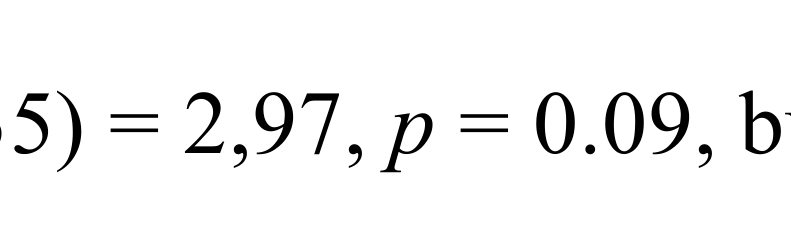
\includegraphics[width=0.85\textwidth]{figures/comma-inset.png}
\caption{The reward statistic on dissertation page~29 (PDF page~37).
The mark between 2 and 97 is a comma.
The \(p\)-value on the same line uses a period.}
\label{fig:comma}
\end{figure}

\begin{figure}[ht]
\centering
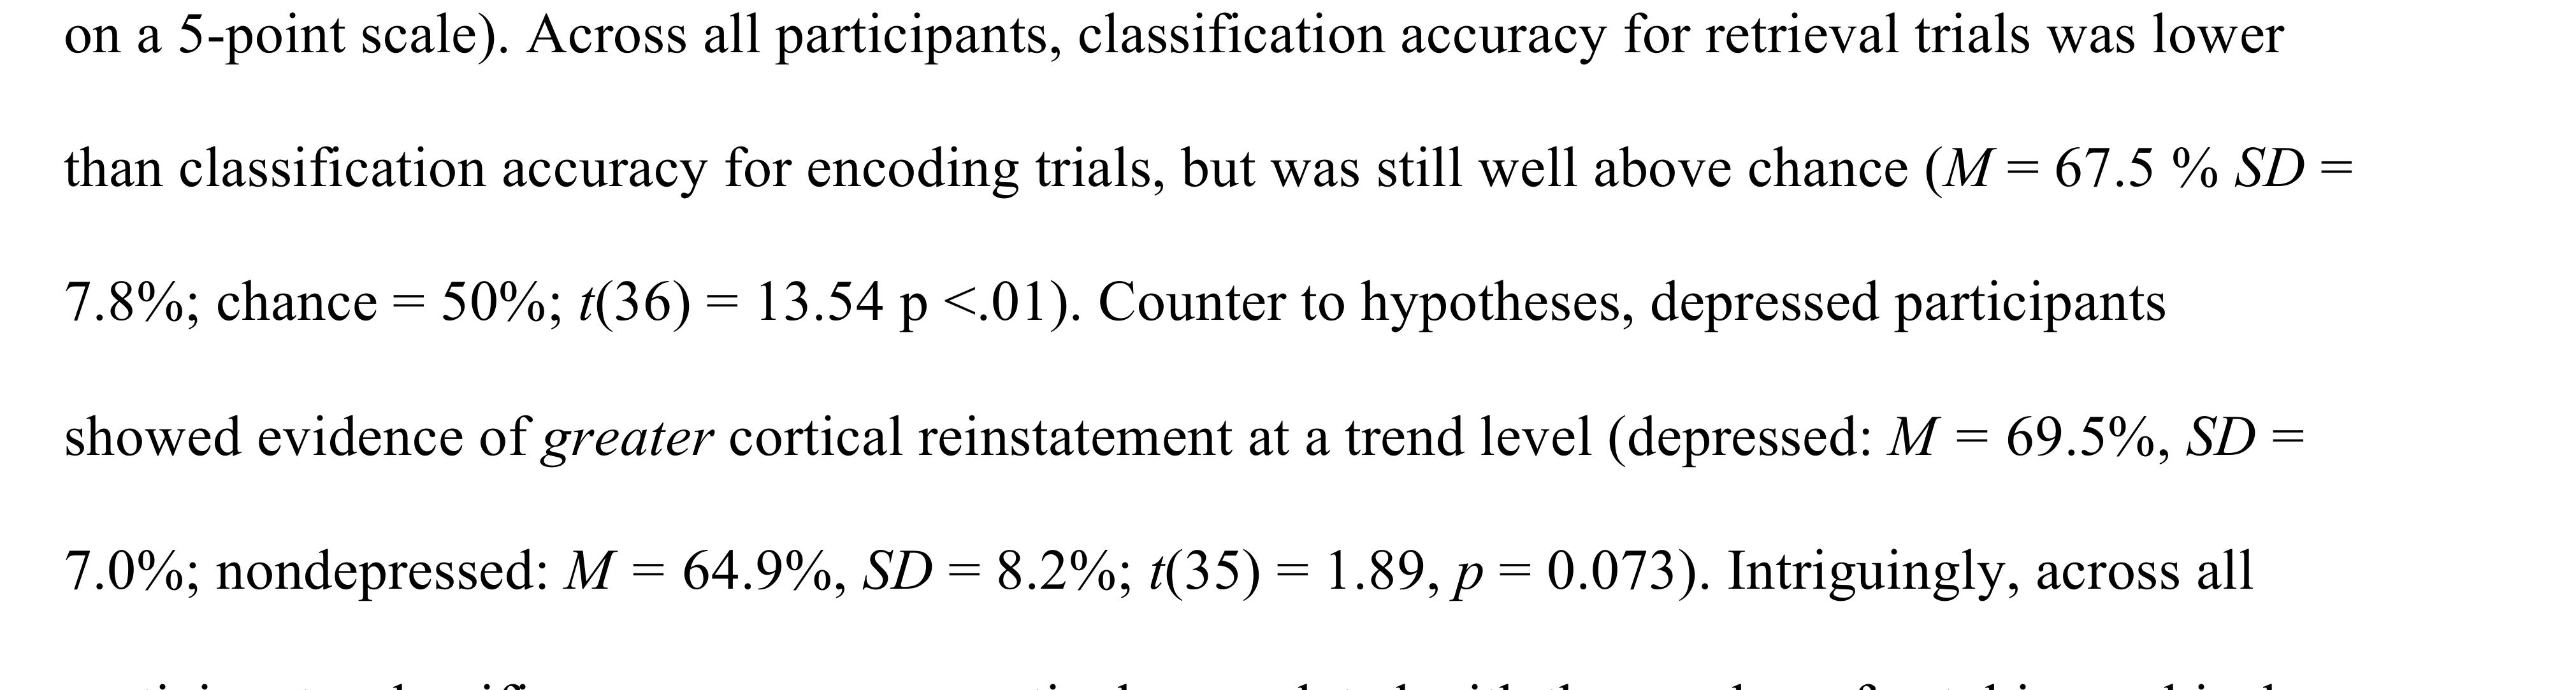
\includegraphics[width=\textwidth]{figures/reinstatement.png}
\caption{Cortical-reinstatement accuracies on dissertation page~30
(PDF page~38).
The above-chance test is \(t(36) = 13.54\).
The group test is \(t(35) = 1.89\), \(p = 0.073\).}
\label{fig:reinstatement}
\end{figure}

Our derived effect sizes, which the dissertation does not print, use the
pooled standard deviation from \srcat{simulation/recompute.R}{37}.
For specific memories, depressed minus nondepressed, Cohen's \(d\) is
\(-0.645\) and Hedges's \(g\) is \(-0.631\).
The 95\% confidence interval for the mean difference is \(-2.08\) to
\(0.04\), which includes 0.
For the Beck inventory at the recruited sizes, \(d = 3.50\).
At the final sizes, \(d = 3.42\).
For negative mood at 20 and 17, \(d = 1.46\).
At 19 and 18, \(d = 1.50\).
For general hits, \(d = 0.518\).
For the group difference in reinstatement accuracy, \(d = 0.607\).
The Hedges factor is \(1 - 3/(4\,\mathrm{df} - 1)\).

\section{What gave us trouble, and how it was resolved}
\label{sec:trouble}

This section answers which gaps closed after the reading, the sample size,
the variance formula, and the page image were checked, in that order.

\subsection{The Beck statistic and the degrees of freedom}
\label{sec:bdi}

The printed claim is one test, \(t(35) = 10.94\).
The moments and the recruited sizes 20 and 19 produce \(t = 10.938\) on 37
degrees of freedom.
The moments and the final sizes 20 and 17 produce \(t = 10.360\) on 35
degrees of freedom.
Welch's \(t\) is \(11.199\) at 20 and 19, and \(11.163\) at 20 and 17.
The second variance formula does not land on \(10.94\).
Figure~\ref{fig:bdi} is the row.
The gap that remains is that no one sample size among these reproduces both
the statistic and the degrees of freedom.
Both readings give \(p < 0.001\).

\begin{figure}[ht]
\centering
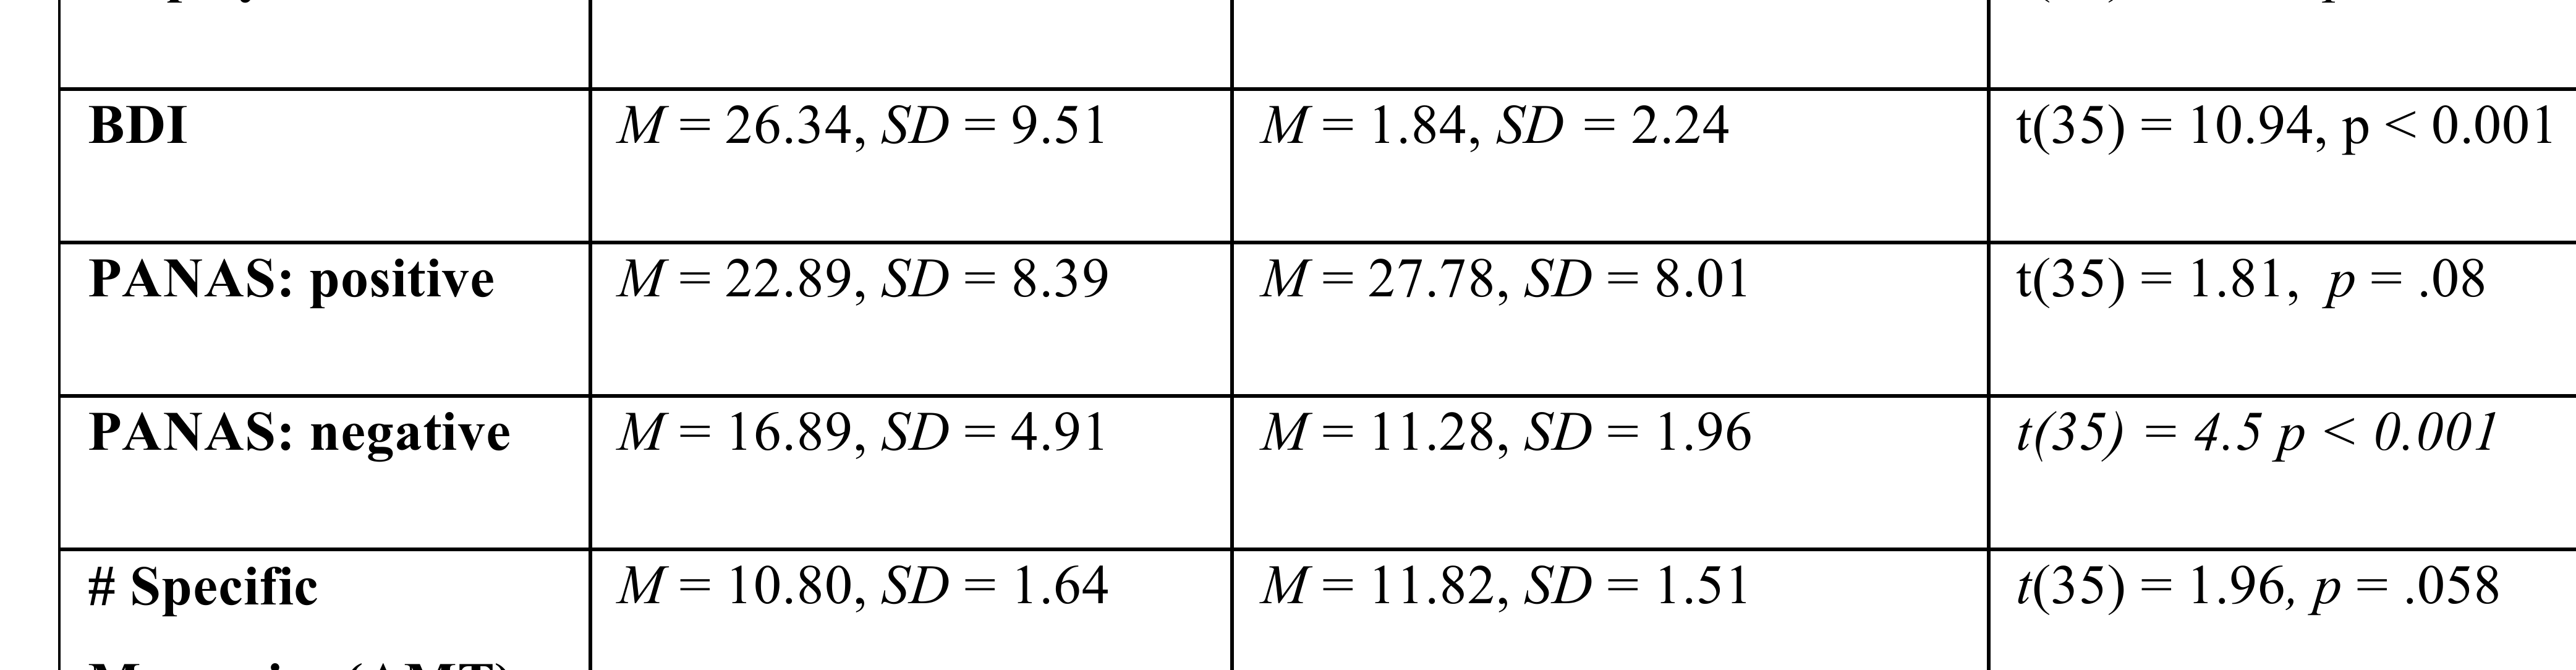
\includegraphics[width=\textwidth]{figures/bdi-panas.png}
\caption{Beck and PANAS rows of dissertation Table~1 (PDF page~54).
The Beck \(t\) is printed on 35 degrees of freedom.
The negative-mood \(t\) is printed as \(4.5\).}
\label{fig:bdi}
\end{figure}

Integer Beck totals make the same split visible.
A 21-item inventory scored 0 to 3 has integer totals from 0 to 63.
\srcat{simulation/recompute.R}{96} finds no integer total whose average
rounds to \(26.34\) at \(n = 20\), and none at \(n = 19\).
The nondepressed mean \(1.84\) is the average of the integer 35 at \(n = 19\),
and it is not an integer average at \(n = 17\).
A prorated Beck score would fall outside that integer check.
The dissertation does not say that any Beck form was prorated.

\subsection{The mood means}
\label{sec:panas}

At the stated final sizes, the positive-mood \(t\) is \(1.804\) against the
printed \(1.81\), and the negative-mood \(t\) is \(4.414\) against the printed
\(4.5\).
The negative-mood half-digit band excludes \(4.5\).
PANAS totals are integers from 10 to 50 when each of ten items is scored 1
to 5.
Neither printed mood mean is an integer average at 20, and the nondepressed
means are not integer averages at 17.
Both depressed means are integer averages at 19 (totals 435 and 321).
Both nondepressed means are integer averages at 18 (totals 500 and 203).
Those sizes sum to 37, so the Student degrees of freedom are 35, which is
the printed degrees of freedom.
On that split the positive-mood \(t\) is \(-1.811\) and the negative-mood
\(t\) is \(4.516\), which prints as \(4.5\).
Turning the split off, and using 20 and 17, returns the gap in the
negative-mood row.
The \(p < 0.001\) conclusion holds on both splits.

\subsection{The comma in the reward statistic}
\label{sec:comma}

The text layer and the 600 dpi page both show \(F(1,35) = 2{,}97\), with a
comma, beside \(p = 0.09\), with a period.
\srcat{paper/figures/crop_pages.py}{66} cuts that mark, and
Figure~\ref{fig:comma} is the cut.
\(F(1,35) = 2.97\) has \(p = .0936\).
\(F(1,35) = 297\) has \(p = 1.1\times 10^{-18}\).
The \(p\)-value selects the reading \(2.97\).
The \(F\) itself is not recomputed from trial outcomes.
The follow-up paired \(t(36) = 1.80\) has \(t^2 = 3.24\), so it is a
different contrast from this \(F\).

\subsection{Handedness and the gender hundredth}
\label{sec:chi}

Figure~\ref{fig:chi} shows the counts.
The gender calculation in \srcat{simulation/recompute.R}{150} is \(0.20783\).
Ordinary two-decimal rounding of that value is \(0.21\).
The page prints \(0.20\).
The continuity-corrected statistic is \(0.016\), so the page is the
uncorrected statistic reported a hundredth lower.
The inequality \(p > 0.1\) holds (\(p = .65\)).
The extra parenthesis after \(0.20\) is on the page.
The handedness counts are 17, 2, and 1 against 17 and 2.
The three-category Pearson statistic is \(0.975\), on 2 degrees of freedom,
and the page prints 1 degree of freedom.
Expected counts in the ambidextrous column are about one half, so the
chi-square tail is a rough approximation there.
The inequality \(p > 0.1\) holds for the three-category test (\(p = .61\))
and for the printed statistic on 1 degree of freedom (\(p = .32\)).

\begin{figure}[ht]
\centering
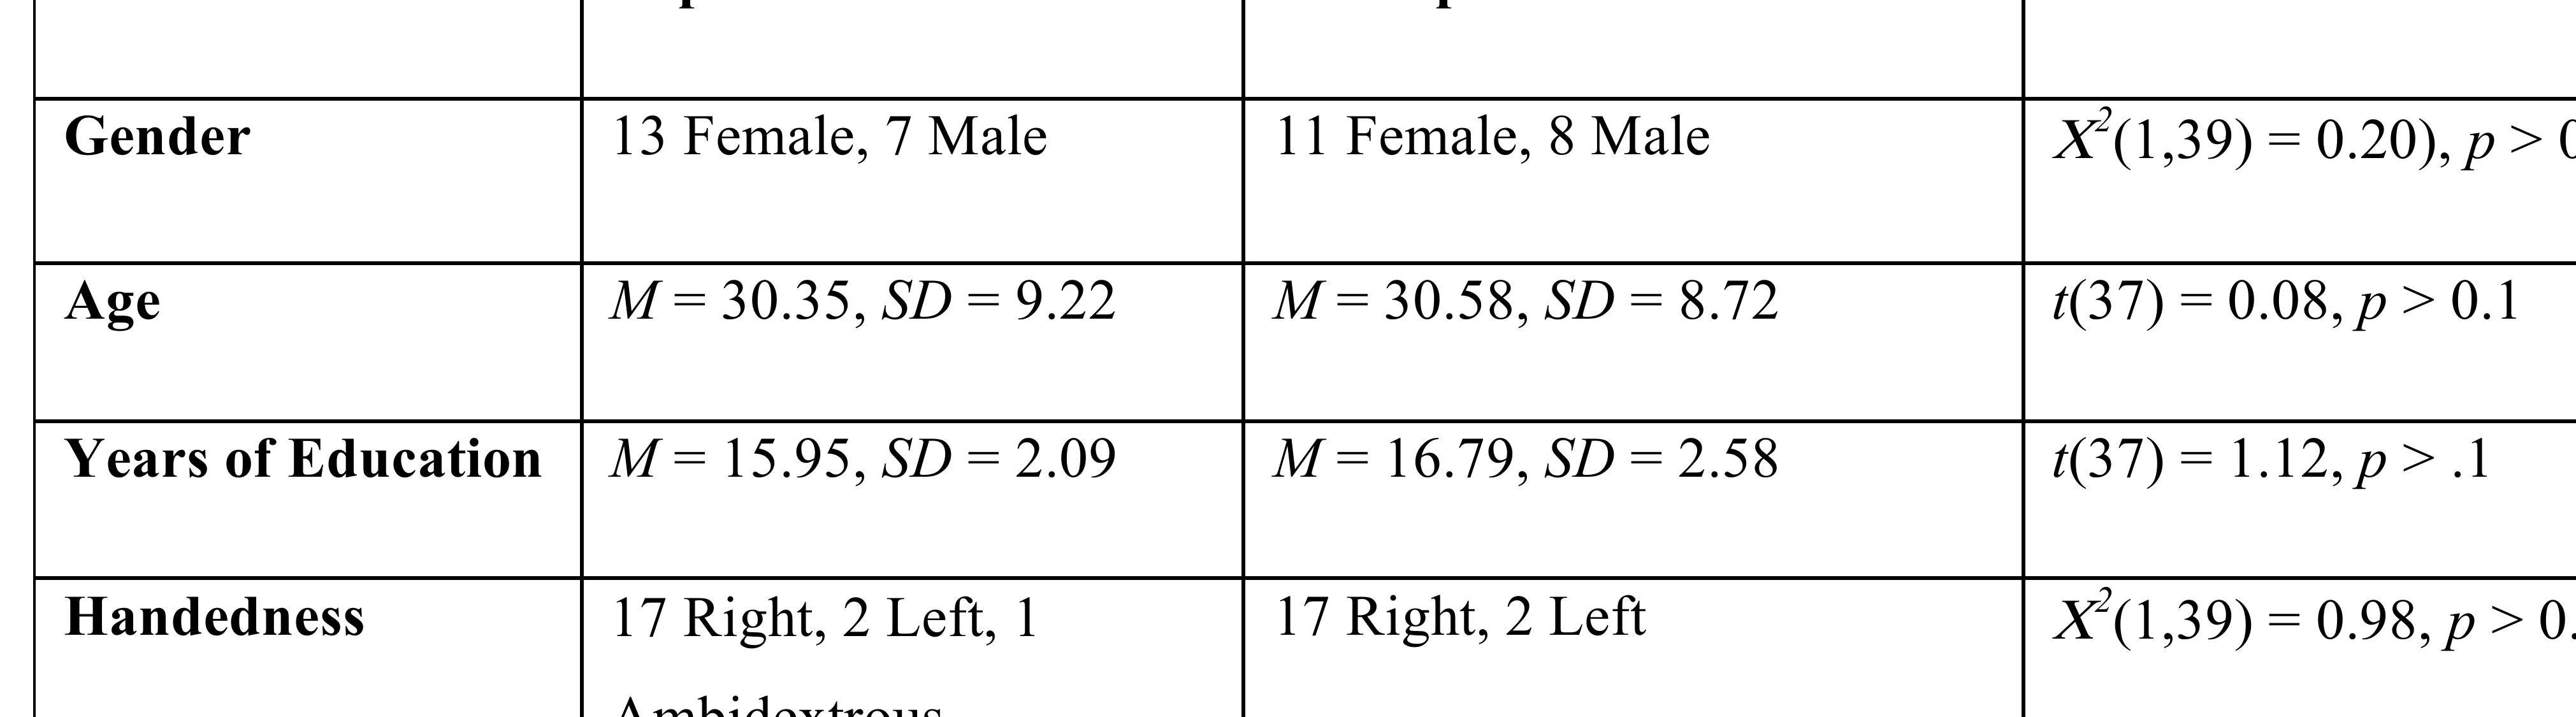
\includegraphics[width=\textwidth]{figures/chi-square.png}
\caption{Gender, age, education, and handedness in dissertation Table~1.
The gender line prints \(\chi^2(1,39) = 0.20\) with an extra parenthesis.
The handedness line prints \(\chi^2(1,39) = 0.98\).}
\label{fig:chi}
\end{figure}

\section{Assumptions}
\label{sec:assumptions}

This section answers which choices the dissertation does not state and
which we supplied.
Each subsection is one choice.
A sample size or a degrees of freedom that the page states is not in this
list.

\subsection{Two-sided tails}

The page prints inequalities and a few exact \(p\)-values, and it does not
say whether the tail is one-sided.
Every \(p\)-value in Table~\ref{tab:compare} is two-sided.
\srcat{simulation/recompute.R}{37} uses \(2\,P(T \ge |t|)\).
One-sided tails would halve those \(p\)-values and would still meet the
printed inequalities for the rows whose conclusion is \(p < .05\),
\(p < .01\), or \(p < 0.001\).

\subsection{Half a unit in the last printed digit}

A printed moment is treated as any value that rounds to it.
A mean or standard deviation printed to two decimals may move by \(0.005\).
A one-decimal number may move by \(0.05\).
\srcat{simulation/recompute.R}{71} evaluates the Student \(t\) on that box.
The negative-cue standard deviation is printed as \(0.8\).
The cue-contrast rows also report the tighter box that reads it as \(0.80\),
and the printed \(t\) values sit in that tighter box as well.
Percent accuracies printed to one decimal use the wider box.

\subsection{Integer instrument totals}

The granularity check assumes the usual integer totals: Autobiographical
Memory Test counts from 0 to 15, and from 0 to 5 within a valence; Beck
totals from 0 to 63; PANAS totals from 10 to 50; Shipley vocabulary from 0
to 40; general hits from 0 to 96.
Age uses the stated inclusion window, 18 to 50 years.
Education uses the stated floor of 12 years and an upper bound of 30 years
that we supplied.
The minimum standard deviation in \srcat{simulation/recompute.R}{111} is the
most equal integers with the required sum.
For every row whose mean is an integer average, the printed standard
deviation is above that minimum.
The output is \src{simulation/out/grim.json}.

\subsection{Mood sample of 19 and 18}

The mood row that matches both printed \(t\) statistics uses 19 depressed
and 18 nondepressed participants.
The dissertation states the final analysis sample as 20 and 17.
The 19-and-18 split is the nearby split on which both PANAS means are
integer averages and both Student statistics print as the page prints them.
It is recorded as a separate row so that the stated-size calculation stays
visible.

\subsection{Correlation sample size}

The correlation lines do not print a degrees of freedom.
The tails use \(N = 37\), the final sample, and, where the missing clarity
ratings could remove the one nondepressed participant, also \(N = 36\).
Both sizes meet the printed inequalities for \(r = -.36\), \(r = -0.33\),
and \(r = .46\).

\section{Ambiguities that were resolved}
\label{sec:resolved}

This section answers which readings are fixed by an artifact.
Each subsection names the script, the output, the command, and the commit
\proofcommit.

\subsection{Student degrees of freedom}

The printed \(t(35)\), \(t(36)\), and \(t(37)\) are the equal-variance
degrees of freedom \(n_1+n_2-2\), or \(n-1\) for a one-sample or paired
\(t\).
\srcat{simulation/recompute.R}{37} is that formula.
Welch's \(t\) is the alternative, and for the Beck inventory it does not
reproduce \(10.94\).
Output: \src{simulation/out/claims.json}.
Command, from the repository root:
\texttt{Rscript formalization/overgeneral-memory/simulation/recompute.R}.

\subsection{The denominator 105}

Figure~\ref{fig:claritydf} prints \(F(1,105)\) for the subsequent-memory
effect in a three-way layout: group, reward, and later hit or miss.
A mixed model with the proper subject-by-memory error would use 35 degrees
of freedom at \(N = 37\).
Thirty-seven participants, each with three within-subject degrees of
freedom, give 111.
The six within-subject terms are reward, memory, their interaction, and
each of those with group.
The residual is \(111 - 6 = 105\).
\srcat{simulation/recompute.R}{238} is that difference.
The same count is 102 at \(N = 36\), so the printed denominator agrees with
keeping all 37 final-sample participants in the clarity analysis.
Output: the \texttt{memory\_F\_df} entry in \src{simulation/out/claims.json}.
Command: the same \texttt{Rscript} invocation.

\begin{figure}[ht]
\centering
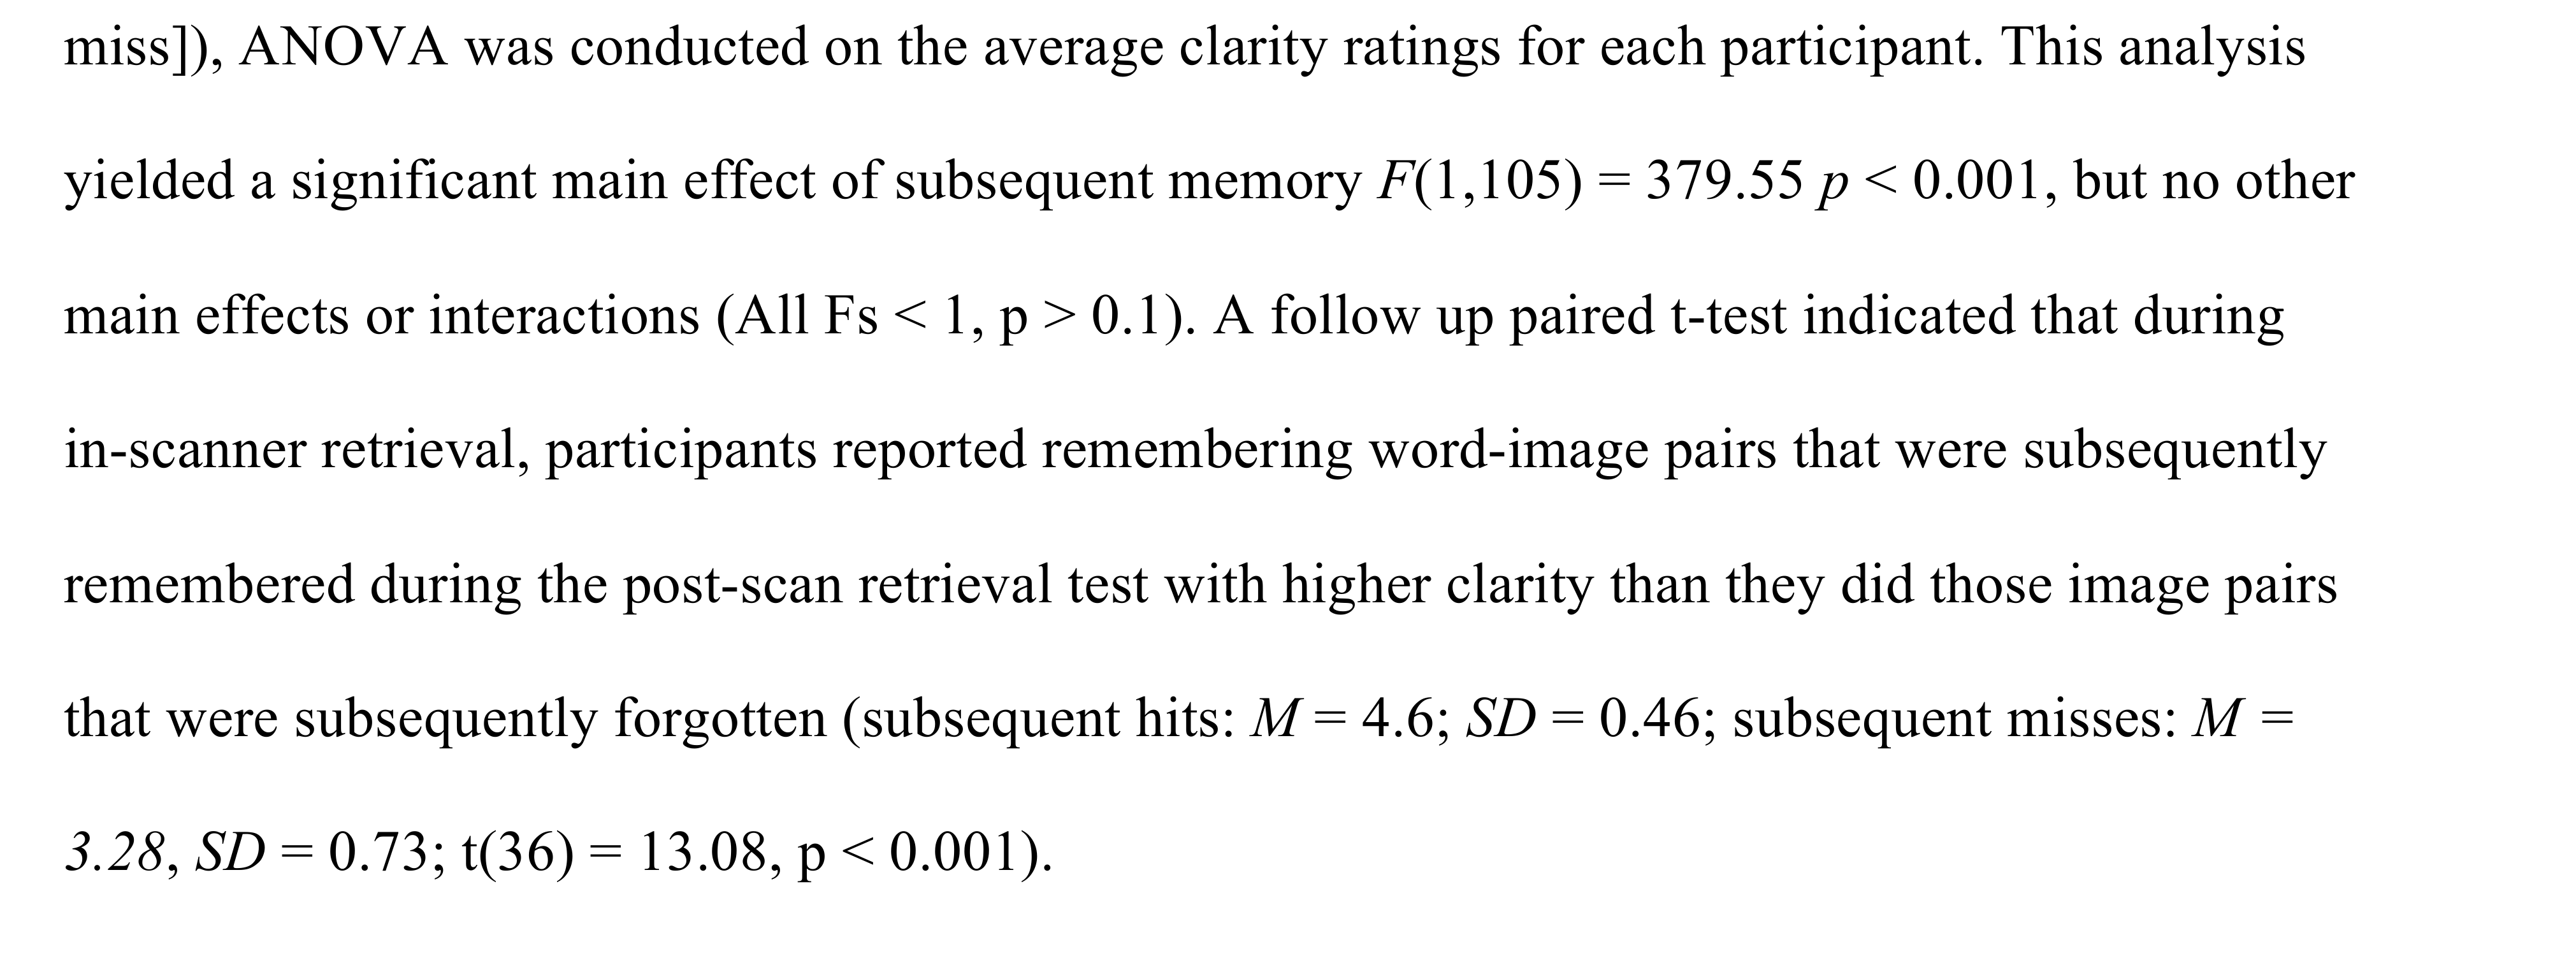
\includegraphics[width=\textwidth]{figures/clarity-df.png}
\caption{Clarity analyses on dissertation page~28 (PDF page~36).
The subsequent-memory effect is printed as \(F(1,105) = 379.55\).
The paired follow-up is \(t(36) = 13.08\).}
\label{fig:claritydf}
\end{figure}

\subsection{The reward comma}

The page image and the text layer agree on a comma in \(2{,}97\).
The \(p\)-value \(0.09\) agrees with \(F = 2.97\) and disagrees with
\(F = 297\).
The crop is \src{paper/figures/comma-inset.png}, from
\srcat{paper/figures/crop_pages.py}{31}.
Command, from the repository root:
\texttt{python3 formalization/overgeneral-memory/paper/figures/crop\_pages.py}
\texttt{--pdf} followed by the local path of the dissertation PDF.

\subsection{Pearson versus Yates}

The gender counts determine \(0.208\) without continuity correction and
\(0.016\) with it.
The page sits a hundredth from the uncorrected statistic.
The continuity-corrected statistic is \(0.016\).
Output: the \texttt{gender} entry in \src{simulation/out/claims.json}.

\section{Small differences that are not replication failures}
\label{sec:small}

This section answers which printed details differ by a hundredth, a
rounding step, or a mark on the page, and whether that difference is a
failure of the test.
None of the items in this list is a failure of the conclusion the page
draws from that test.

The center of the specificity \(t\) is \(1.95\), one step from the printed
\(1.96\), and \(1.96\) is inside the half-digit band.
The square of the center is \(3.82\), and the printed \(F\) is \(3.84\), the
square of \(1.96\).
The gender statistic \(0.208\) is printed as \(0.20\), with an extra
parenthesis after the number.
The Shipley \(t\) at the integer-consistent sizes is \(0.557\), printed as
\(0.55\).
The clarity means are both printed as \(3.9\), and the exact-\(3.9\) \(t\) is
0, while \(0.17\) is inside the one-decimal band.
The encoding-classification center is \(1.24\) against the printed \(1.26\),
inside the percentage band.
The above-chance reinstatement center is \(13.65\) against the printed
\(13.54\), inside the percentage band.
The group reinstatement center is \(1.84\) with \(p = .074\), against
\(t = 1.89\) and \(p = 0.073\).
The voxel-count \(t\) is \(0.075\), which rounds to the printed \(0.07\).
The methods heading ``Cortical Reinstatemet'' and the word ``furisform'' in
the classification paragraph are spelling on the page.
Table~2 prints a 21-voxel cluster at the boundary of the stated rule
``larger than 21 voxels.''
That boundary is a wording detail of a cluster list we did not recompute.

\section{What remains unresolved}
\label{sec:open}

This section answers which printed claims stay open, and what was tried on
them.

The right prefrontal cluster, and every other cluster table, stays open.
The dissertation's univariate results are AFNI \texttt{3dMEMA} maps.
No image, no bucket file, and no table of participant-level region betas is
in the repository record or in the places in Section~\ref{sec:availability}.
The correlation \(r = .46\) was checked only as a tail probability.
The same limit covers encoding maps, reward maps, and the classifier
accuracies as neural quantities: the printed percentages were checked as
moments, and the images were not reclassified.

The Beck row stays split.
Recruited sizes reproduce the \(t\) and final sizes reproduce the degrees of
freedom.
Integer totals reproduce the nondepressed mean at the recruited size and do
not reproduce the depressed mean \(26.34\).
The item scores would close this.
Welch's \(t\) was the second formula, and it did not close it.

The reaction-time degrees of freedom stay one above the hits tests in the
same paragraph.
\(F(1,36)\) is the equal-variance error for a two-group sample of 38, or
\(N-1\) for a sample of 37.
The dissertation does not say that a removed participant was put back for
the reaction times.
The three \(F\) values were not recomputed, because the reaction times are
not printed.
Their tail inequalities hold.

The valence \(F\), the interaction \(F\), the specific-hits \(F\), and the
reward \(F\) stay as tail checks.
Cell means and the within-subject correlations are not printed.
The paired clarity \(t\) and the paired reward \(t\) are feasible given the
marginal moments, and they are not identified by those moments.

The exclusion sentence and the clarity degrees of freedom describe different
samples.
The text says one nondepressed participant lacked clarity ratings and was
left out of analyses that used those ratings.
The printed clarity tests use \(t(35)\), \(t(36)\), and \(F(1,105)\), which
agree with \(N = 37\).
The denominator arithmetic in Section~\ref{sec:resolved} uses that \(N\).
Which of the two the clarity means actually used is open.
A superscript 1 follows the PANAS sentence in the participants section, and
the file contains no footnote text for that mark, so whatever it qualified
is not in the PDF we read.

An unquoted GitHub code query for the author and the word autobiographical
returned unrelated repositories.
A quoted search for the dissertation title returned HTTP 429 and did not
finish.
That quoted search is unfinished in Section~\ref{sec:availability}.

\section{Code and source availability}
\label{sec:availability}

This section answers where the dissertation, the code, and the images were
sought on 29 October 2026 (UTC).
Table~\ref{tab:ledger} is that ledger.
``Not available'' is not the summary: the PDF was obtained, and several
later rows did not obtain a second file.

\begin{footnotesize}
\begin{longtable}{@{}L{0.34\textwidth}L{0.16\textwidth}L{0.42\textwidth}@{}}
\caption{Places checked for the dissertation, for code, and for images.}
\label{tab:ledger}\\
\toprule
Place checked & UTC date & Result \\
\midrule
\endfirsthead
\toprule
Place checked & UTC date & Result \\
\midrule
\endhead
Dissertation PDF, Stanford stacks
\url{https://stacks.stanford.edu/file/cv880bv1650/Sorenson_Dissertation_To_Submit-augmented.pdf}
& 2026-10-29 &
Obtained. 91 pages, 3{,}233{,}141 bytes, sha256
\sha{4debc9f5551d51ae00a5b6987c3c572a9c7221f6ab631928558c8c1f6b8414d6}.
The text names no code deposit. \\
PURL and Cocina record
\url{https://purl.stanford.edu/cv880bv1650}
& 2026-10-29 &
One file, the PDF. Download is world. License CC BY-NC 3.0. \\
SearchWorks \url{https://searchworks.stanford.edu/view/11391835}
& 2026-10-29 &
Bot challenge page. No catalog body. The stacks PDF was already in hand. \\
ProQuest dissertation search for the title
& 2026-10-29 &
HTTP 302, fifty redirects, no file. \\
OpenAlex author \texttt{A5007153948} and a title search
& 2026-10-29 &
The author record lists one 2019 arXiv paper and does not list this
dissertation. No DOI for the dissertation on that record. \\
Crossref, ``Memory for novel positive information''
& 2026-10-29 &
DOI \texttt{10.1080/02699931.2013.866936}, 2014, a different title.
Full text not retrieved. Not used for these tests. \\
OSF node titles for this study
& 2026-10-29 &
``overgeneral autobiographical'' returned four other papers.
``Gotlib memory'' and ``PARC paired associates'' returned no nodes.
\texttt{/v2/search/} returned HTTP 404. \\
Zenodo, quoted name ``James Eric Sorenson''
& 2026-10-29 &
Zero records. \\
GitHub users, ``James Eric Sorenson''
& 2026-10-29 &
Zero users. Accounts under the surname Sorenson are other people
(a media company, an Eric Sorenson, a Lockheed engineer).
Those repositories were not cloned. \\
GitHub code search
& 2026-10-29 &
Unquoted query: 280 hits, first page unrelated.
Quoted dissertation title: HTTP 429, not finished. \\
GitLab projects, ``sorenson autobiographical''
& 2026-10-29 &
Empty list. \\
OpenNeuro \texttt{advancedSearch}, depression and autobiographical
& 2026-10-29 &
No datasets. A keywords-only autobiographical query returned other
studies (\texttt{ds003511}, \texttt{ds000210}, \texttt{ds001618}, and
others). \\
NDA search API and query page
& 2026-10-29 &
API path HTTP 404. Query page HTTP 302. No dataset record retrieved. \\
\bottomrule
\end{longtable}
\end{footnotesize}

The dissertation names Praat 5.4.08 for spoken reaction times, AFNI for the
univariate models, FreeSurfer for the anatomical segmentation, and nilearn
with scikit-learn for the classifier.
Those are programs, not a deposit of this study's scripts or images.
We did not run them.

\section{Next steps}
\label{sec:next}

This section answers what would close the open rows.
The participant-level Autobiographical Memory Test scores, Beck and PANAS
item totals, and the paired-associate hit counts would decide whether the
mood rows are 20 and 17 or 19 and 18, whether the Beck \(t\) and its degrees
of freedom come from one sample, and whether the paired \(t\) values are the
printed ones.
The AFNI \texttt{3dMEMA} buckets, or the right middle frontal gyrus betas
that were correlated with specificity, would decide the cluster contrast and
the value of \(r = .46\), not only its tail.
A session log would name the program that printed the behavioral \(F\) tests.
A finished GitHub code search, after the rate limit, is the remaining
public-code check.

\section{Artifacts}
\label{app:artifacts}

This appendix answers where each claim lives and which command writes it.
The dissertation PDF is local and gitignored.
Its sha256 is
\sha{4debc9f5551d51ae00a5b6987c3c572a9c7221f6ab631928558c8c1f6b8414d6}.

\begin{itemize}
\item All comparison rows.
File \src{simulation/out/claims.json} and \src{simulation/out/claims.csv}.
Command: \texttt{Rscript} \src{simulation/recompute.R}.
\item Integer-score checks.
File \src{simulation/out/grim.json}.
The same command.
\item Derived \(d\), \(g\), and confidence intervals.
File \src{simulation/out/derived.json}.
The same command.
\item R version.
File \src{simulation/out/sessionInfo.txt}.
The same command.
\item Page crops.
Directory \src{paper/figures/}.
Command: \texttt{python3} \srcat{paper/figures/crop_pages.py}{72}
with \texttt{--pdf} set to the local dissertation file.
\end{itemize}

\begin{thebibliography}{9}

\bibitem{sorenson2015}
James Eric Sorenson.
\emph{Overgeneral autobiographical memory in major depressive disorder is
associated with abnormal neural activity during retrieval}.
Ph.D.\ dissertation, Stanford University, 2015.
\url{https://purl.stanford.edu/cv880bv1650}.

\bibitem{rcore}
R Core Team.
\emph{R: A Language and Environment for Statistical Computing}.
R Foundation for Statistical Computing, Vienna, Austria, 2024.
R version 4.3.3.
\url{https://www.R-project.org/}.

\bibitem{jsonlite}
Jeroen Ooms.
The jsonlite package: A practical and consistent mapping between JSON data
and R objects.
\emph{arXiv:1403.2805}, 2014.
jsonlite 1.8.8.
\url{https://cran.r-project.org/package=jsonlite}.

\bibitem{poppler}
Poppler developers.
Poppler 24.02.0.
\url{https://poppler.freedesktop.org/}.

\bibitem{python}
Python Software Foundation.
Python 3.12.3.
\url{https://www.python.org/}.

\bibitem{pillow}
Jeffrey A.\ Clark and contributors.
Pillow 10.2.0.
\url{https://python-pillow.org/}.

\bibitem{texlive}
\TeX\ Live developers.
pdf\TeX\ 3.141592653-2.6-1.40.25, \TeX\ Live 2023.
\url{https://tug.org/texlive/}.

\end{thebibliography}

\end{document}
